\documentclass{report}

\usepackage{graphicx}

\usepackage{pdfpages} 

\usepackage{amsmath}
\usepackage{listings}
\usepackage{color} %red, green, blue, yellow, cyan, magenta, black, white
\definecolor{mygreen}{RGB}{28,172,0} % color values Red, Green, Blue
\definecolor{mylilas}{RGB}{170,55,241}


\title{\textbf{Computational Mathematics - Assignment 1}\\Owen Burke, 15316452}
\begin{document}

    \lstset{language=Matlab,%
    %basicstyle=\color{red},
    breaklines=true,%
    morekeywords={matlab2tikz},
    keywordstyle=\color{blue},%
    morekeywords=[2]{1}, keywordstyle=[2]{\color{black}},
    identifierstyle=\color{black},%
    stringstyle=\color{mylilas},
    commentstyle=\color{mygreen},%
    showstringspaces=false,%without this there will be a symbol in the places where there is a space
    numbers=left,%
    numberstyle={\tiny \color{black}},% size of the numbers
    numbersep=9pt, % this defines how far the numbers are from the text
    emph=[1]{for,end,break},emphstyle=[1]\color{red}, %some words to emphasise
    %emph=[2]{word1,word2}, emphstyle=[2]{style},    
}







    \maketitle
    \section*{\hfil Question 2.31 \hfil}
    Write a user-defined MATLAB function that calculates the determinant of a square (n x n) matrix, where n can be 2, 3, or 4. For function name and arguments, use D =  Determinant (A). 
    The input argu­ment A is the matrix whose determinant is calculated. The function Determinant should first check if the matrix is square. If it is not, the output D should be the
    message "The matrix must be square." Use Determinant to calculate the determinant of the following two matrices: 
        \subsection*{}
            \begin{figure}[h!]
                        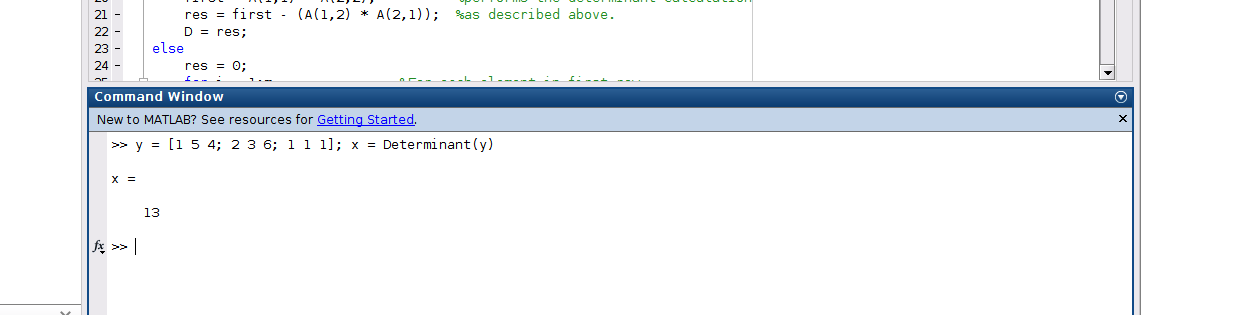
\includegraphics[width=\linewidth]{Determinant_a).png}
                        \caption{Determinant a)}
                        \label{fig:Determinant a)}
            \end{figure}

                    

            \begin{figure}[h!]
                        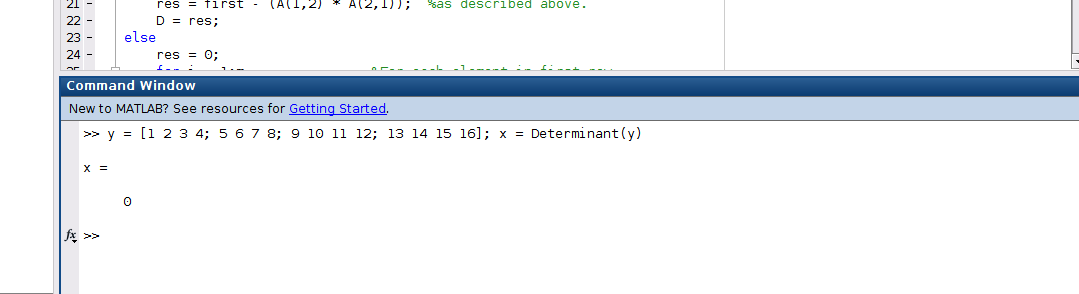
\includegraphics[width=\linewidth]{Determinant_b).png}
                        \caption{Determinant b)}
                        \label{fig:Determinant b)}
            \end{figure}

                    


		\subsection*{a) $\begin{bmatrix}
            1 & 5 & 4\\
            2 & 3 & 6\\
            1 & 1 & 1\\
            \end{bmatrix}$ b) $\begin{bmatrix}
                1 & 2 & 3 & 4\\
                5 & 6 & 7 & 8\\
                9 & 10 & 11 & 12\\
                13 & 14 & 15 & 16\\
                \end{bmatrix}$}


                \lstinputlisting{Determinant.m}
    
                  












    \section*{\hfil Question 3.2 \hfil}
    Determine the root of f (x) = x - 2e\textsuperscript{-x} by:
        \subsection*{a) Using the bisection method. Start with a = 0 and  b = 1, and carry out the first three iterations.}
                \textbf{1\textsuperscript{st} iteration:}\\\\
                Given a = 0 and b = 1, find the first numerical solution given by 

                \begin{center}
                    X\textsubscript{NS1} = $\frac{a + b}{2}$ = $\frac{0 + 1}{2}$ = 0.5
                \end{center}

                Now, Determine whether the true solution is between a and X\textsubscript{NS1} or between X\textsubscript{NS1} and b.\\
                This is done by checking the sign of the product f(a)f(X\textsubscript{NS1}).\\
                If the product is positive, then the true solution lies between X\textsubscript{NS1} and b.\\
                Otherwise, it is between a and X\textsubscript{NS1}.\\

                \begin{center}
                    (0-2e\textsuperscript{-(0)}) * ($\frac{1}{2}$-2e\textsuperscript{-($\frac{1}{2}$)}) = 1.426
                \end{center}

                As this result is positive, we know that the true solution lies between X\textsubscript{NS1} and b,
                so we make a = X\textsubscript{NS1} and let b = b and we repeat for the next iteration with the same process.\\\\

                \textbf{2\textsuperscript{nd} iteration:}\\\\

                Given a = 0.5, b = 1

                \begin{center}
                    X\textsubscript{NS2} = $\frac{a + b}{2}$ = $\frac{0.5 + 1}{2}$ = 0.75
                \end{center}

                Determine which sub-interval contains the true solution

                \begin{center}
                    (0.5-2e\textsuperscript{-(0.5)}) * (0.75-2e\textsuperscript{-(0.75)}) = 0.139
                \end{center}

                As this result is positive, we know that the true solution lies between X\textsubscript{NS2} and b,
                so we make a = X\textsubscript{NS2} and let b = b and we repeat for the next iteration with the same process.\\\\

                \textbf{3\textsuperscript{rd} iteration:}\\\\

                Given a = 0.75, b = 1

                \begin{center}
                    X\textsubscript{NS3} = $\frac{a + b}{2}$ = $\frac{0.75 + 1}{2}$ = $\frac{7}{8}$
                \end{center}

                Determine which sub-interval contains the true solution

                \begin{center}
                    (0.75-2e\textsuperscript{-(0.75)}) * ($\frac{7}{8}$-2e\textsuperscript{-($\frac{7}{8}$)}) = -0.008
                \end{center}

                As this result is negative, we know that the true solution lies between a and X\textsubscript{NS3},
                so we make a = a and let b = X\textsubscript{NS3} and we get the half way point between these two values as our final numerical solution.

                \begin{center}
                    X\textsubscript{FNS} = $\frac{a + b}{2}$ = $\frac{0.75 + 0.875}{2}$ = 0.8125
                \end{center}



        \subsection*{b) Using the secant method. Start with the two points, x\textsubscript{1} = 0 and x\textsubscript{2} = 1, and carry out the first three iter­ations.}
            \textbf{1\textsuperscript{st} iteration:}\\\\
            Given x\textsubscript{1} = 0 and x\textsubscript{2} = 1,\\
            using the identity (for the slope of the secant containing (x\textsubscript{1}f(x\textsubscript{1})), 
            (x\textsubscript{2}f(x\textsubscript{2})), (x\textsubscript{3}f(x\textsubscript{3}))) : 

            \begin{center}
                $\frac{f(x\textsubscript{1}) - f(x\textsubscript{2})}{x\textsubscript{1} - x\textsubscript{2}}$
            \end{center}

            solve for x\textsubscript{3}

            \begin{center}
                x\textsubscript{3} = x\textsubscript{2} - $\frac{f(x\textsubscript{2})(x\textsubscript{1} - x\textsubscript{2})}{f(x\textsubscript{1}) - f(x\textsubscript{2})}$
            \end{center}


            This is given as 

            \begin{center}
                x\textsubscript{3} = 1 - $\frac{(0.264)(1 - 0)}{(-2) - (0.264)}$ = 1.117
            \end{center}

            Now we use (x\textsubscript{2}f(x\textsubscript{2})), (x\textsubscript{3}f(x\textsubscript{3})) as points defining a new secant
             and repeat step 2.\\\\













             \textbf{2\textsuperscript{nd} iteration:}\\\\
            Given x\textsubscript{2} = 1 and x\textsubscript{3} = 1.117,\\

            solve for x\textsubscript{4}

            \begin{center}
                x\textsubscript{4} = x\textsubscript{3} - $\frac{f(x\textsubscript{3})(x\textsubscript{2} - x\textsubscript{3})}{f(x\textsubscript{2}) - f(x\textsubscript{3})}$
            \end{center}


            This is given as 

            \begin{center}
                x\textsubscript{4} = 1.117 - $\frac{(0.462)(1 - 1.117)}{(0.264) - (0.462)}$ = 0.844
            \end{center}

            Now we use (x\textsubscript{3}f(x\textsubscript{3})), (x\textsubscript{4}f(x\textsubscript{4})) as points defining a new secant
             and repeat step 2.\\\\








             \textbf{3\textsuperscript{rd} iteration:}\\\\
             Given x\textsubscript{3} = 1.117 and x\textsubscript{4} = 0.844,\\
 
             solve for x\textsubscript{5}
 
             \begin{center}
                 x\textsubscript{5} = x\textsubscript{4} - $\frac{f(x\textsubscript{4})(x\textsubscript{3} - x\textsubscript{4})}{f(x\textsubscript{3}) - f(x\textsubscript{4})}$
             \end{center}
 
 
             This is given as 
 
             \begin{center}
                 x\textsubscript{5} = 0.844 - $\frac{(-0.016)(1.117 - 0.844)}{(0.462) - (-0.016)}$ = 0.853
             \end{center}
 
             Final numerical solution after three iterations : x = 0.853





























                


        \subsection*{c) Using Newton's method. Start at x\textsubscript{1} = 1 and carry out the first three iterations.}
             Newton's method approximates the solution initially as the intercept of the tangent to the function, at an initial guess-point, 
             with the x −axis. Subsequent iterations approximate the solution as the intercept of the tangent to the function, at the point 
             defined by the previous estimate, with the x −axis. Note that it does not necessarily converge.\\\\

             Given x\textsubscript{1} = 1, our starting point is (x\textsubscript{1},f(x\textsubscript{1})) = (1, 0.264).\\
             Using the identity for slope of the tangent at (x\textsubscript{1},f(x\textsubscript{1})) :
             
             \begin{center}
                 f'(x\textsubscript{1}) = $\frac{f(x\textsubscript{1}) - 0}{x\textsubscript{1} - x\textsubscript{2}}$
             \end{center}

             Solve for x\textsubscript{2} using : 

             \begin{center}
                x\textsubscript{2} = x\textsubscript{1} - $\frac{f(x\textsubscript{1})}{f'(x\textsubscript{1})}$
            \end{center}

            and repeat step 2 iteratively using the formula:


            \begin{center}
                x\textsubscript{i+1} = x\textsubscript{i} - $\frac{f(x\textsubscript{i})}{f'(x\textsubscript{i})}$
            \end{center}


            To begin we must find f'(x).\\\\
            f'(x) = $\frac{dy}{dx}$, where y = f(x)\\\\
            f'(x) = $\frac{d}{dx}$ (x-2e\textsuperscript{-x})\\\\
            f'(x) = $\frac{d(x)}{dx}$ - 2 * $\frac{d(e\textsuperscript{-x})}{dx}$\\\\
            f'(x) = 1 - 2 * (-e\textsuperscript{-x})\\\\
            f'(x) = 1 + 2e\textsuperscript{-x}\\\\

            \textbf{1\textsuperscript{st} iteration:}\\\\
            \begin{center}
                x\textsubscript{2} = 1 - $\frac{0.264}{1+2e\textsuperscript{-(1)}}$ = 1 - $\frac{0.264}{1.736}$ = $\frac{184}{217}$    
            \end{center}

            \textbf{2\textsuperscript{nd} iteration:}\\\\
            \begin{center}
                x\textsubscript{3} = $\frac{184}{217}$ - $\frac{-0.009}{1.857}$ = 0.853    
            \end{center}

            \textbf{3\textsuperscript{rd} iteration:}\\\\
            \begin{center}
                x\textsubscript{4} = 0.853 - $\frac{0.0007}{1.852}$ = 0.853    
            \end{center}

            Final numerical solution after three iterations : x = 0.853
            












































































    \section*{\hfil Question 4.24 \hfil}
    Write a user-defined MATLAB function that determines the inverse of a matrix using the Gauss-Jor­dan method. For the function name and arguments use Ainv =Inverse (A), where A is the 
    matrix to be inverted, and Ainv is the inverse of the matrix. Use the Inverse function to calculate the inverse of:

    \subsection*{}
    \begin{figure}[h!]
                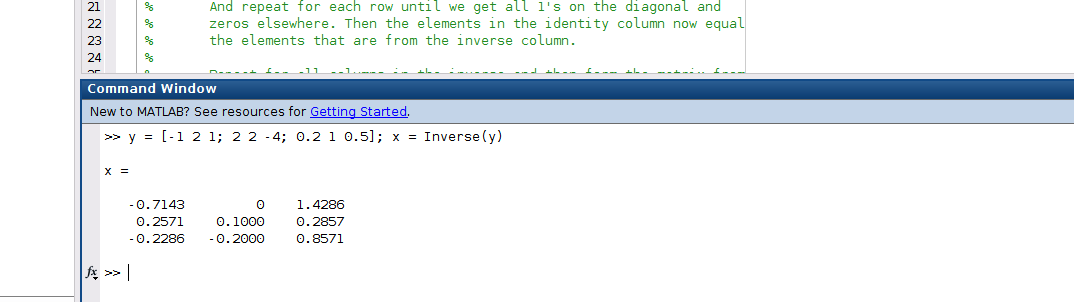
\includegraphics[width=\linewidth]{Inverse_a).png}
                \caption{Inverse a)}
                \label{fig:Inverse a)}
    \end{figure}

            

    \begin{figure}[h!]
                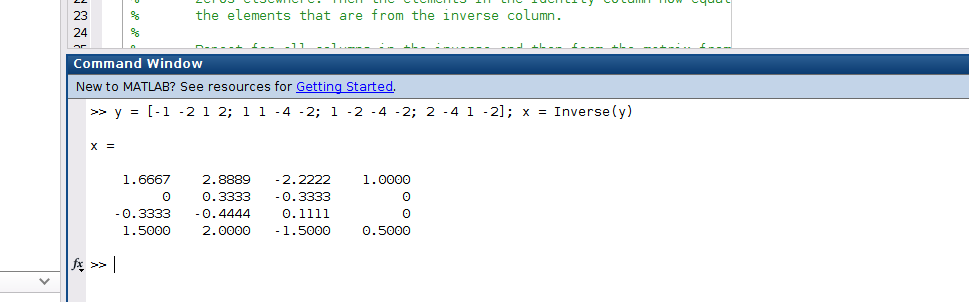
\includegraphics[width=\linewidth]{Inverse_b).png}
                \caption{Inverse b)}
                \label{fig:Inverse b)}
    \end{figure}


        \subsection*{a) $\begin{bmatrix}
            -1 & 2 & 1\\
            2 & 2 & -4\\
            0.2 & 1 & 0.5\\
            \end{bmatrix}$ b) $\begin{bmatrix}
                -1 & -2 & 1 & 2\\
                1 & 1 & -4 & -2\\
                1 & -2 & -4 & -2\\
                2 & -4 & 1 & -2\\
                \end{bmatrix}$}
            
            
                \lstinputlisting{Inverse.m}


























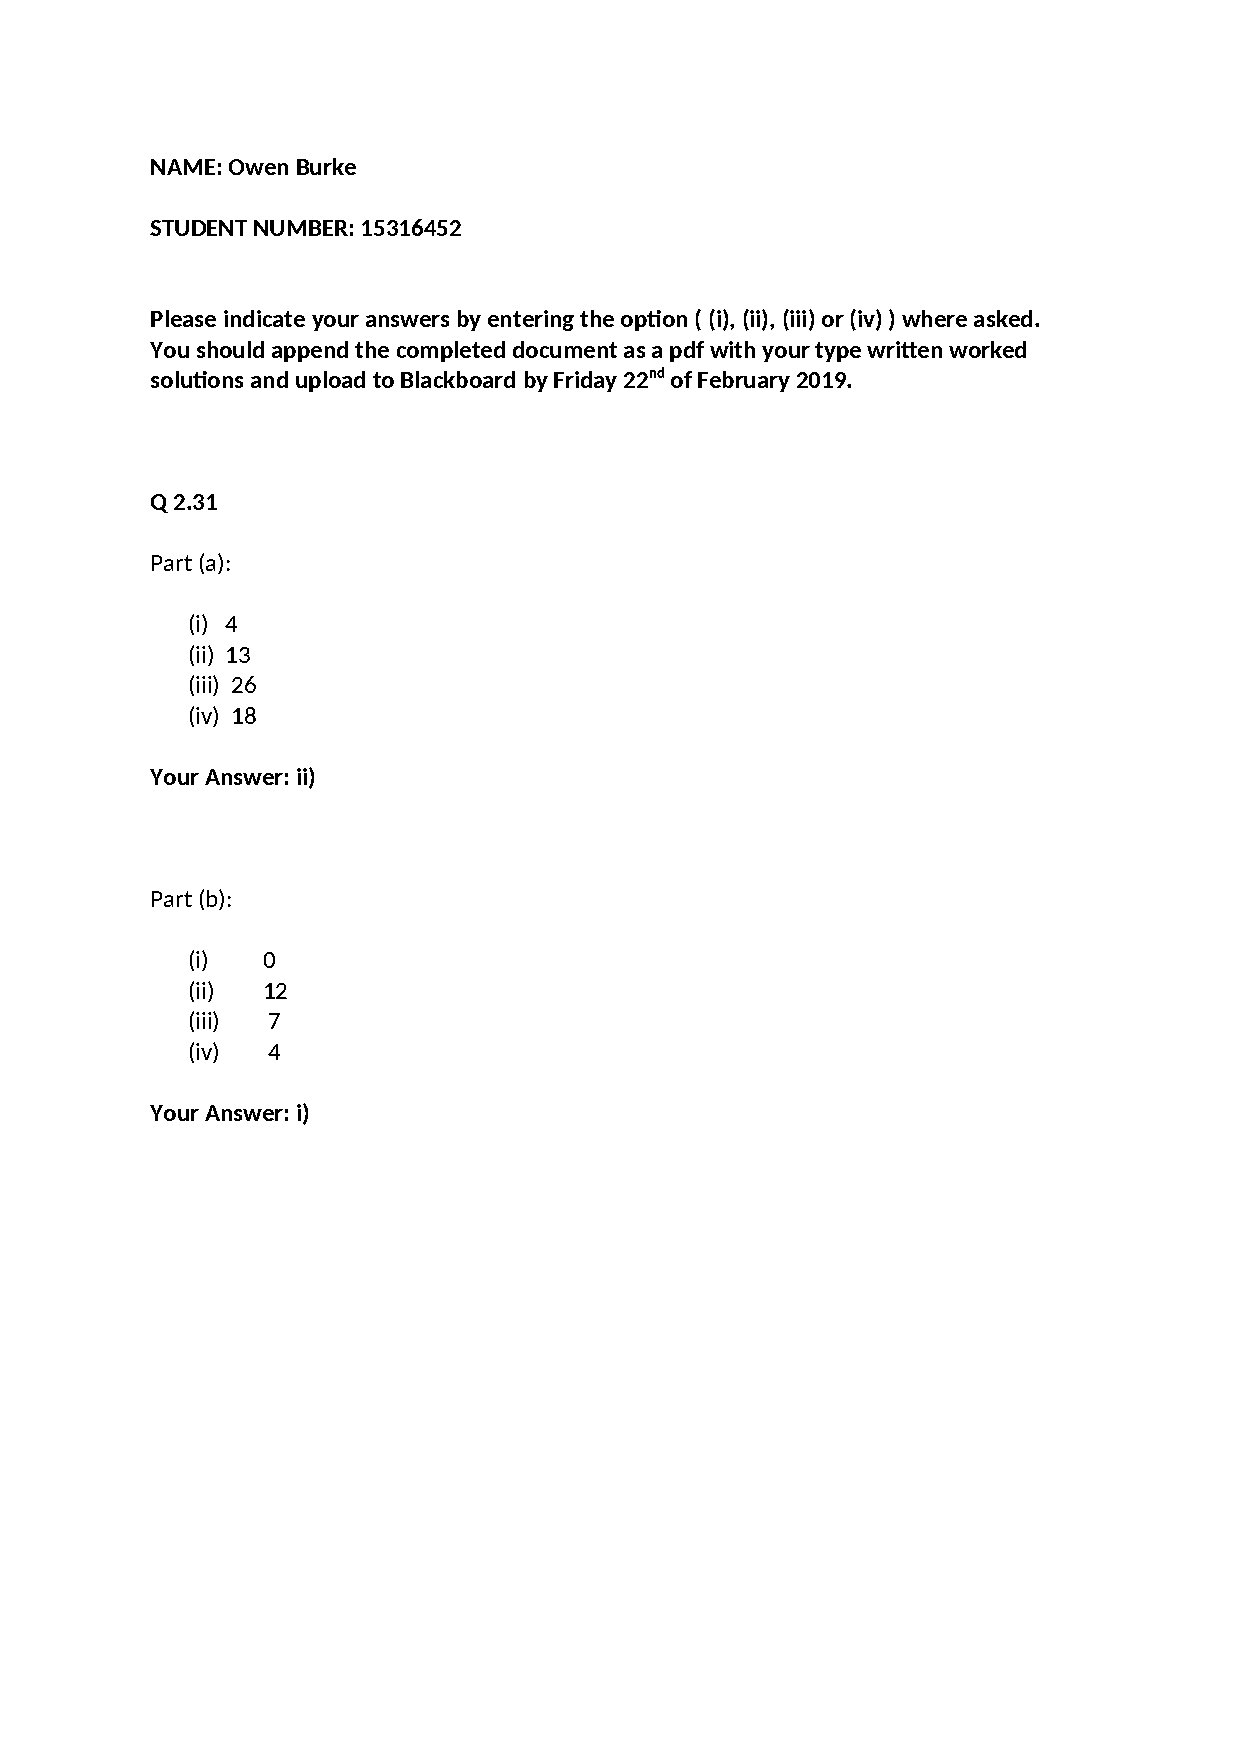
\includepdf[page=-]{CS3081_Assignment_1_Multichoice.pdf}

\end{document}